\documentclass{article}
\usepackage{graphicx} 
\usepackage{pgf-pie}
\usepackage[colorlinks=true, urlcolor=blue]{hyperref}

\title{Logistics : CS213 and CS293}
\author{}
\date{}

\begin{document}

\maketitle

\section{Course Website}
\subsection{CS213}
Lecture Slides : \\\url{https://robin.bodhi.cse.iitb.ac.in/courseware/course/195/content/multimedia/coursecontent/}
\subsection{CS293}
Labs : \\
\url{https://robin.bodhi.cse.iitb.ac.in/courseware/course/195/content/labs}
\\\\
Lab seat mapping : \\\url{https://bit.ly/A26-DSA-Mapping}
\newpage
\section{Grade Distribution}
\subsection{CS213 (Theory)}
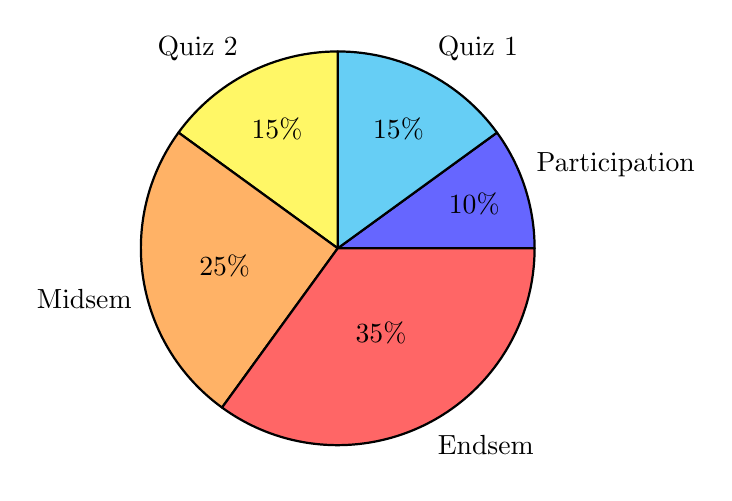
\begin{tikzpicture}
  \pie[radius=2.5]{10/Participation, 15/Quiz 1, 15/Quiz 2, 25/Midsem, 35/Endsem}
\end{tikzpicture}
\subsection{CS293 (Lab)}
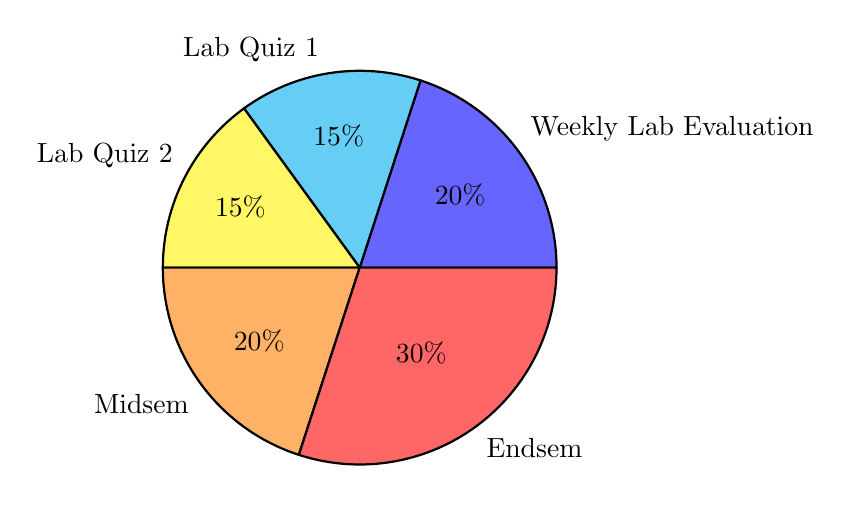
\begin{tikzpicture}
  \pie[radius=2.5]{20/Weekly Lab Evaluation, 15/Lab Quiz 1, 15/Lab Quiz 2, 20/Midsem, 30/Endsem}
\end{tikzpicture}



\end{document}
